\section{GIAO TIẾP VÀ BẢO MẬT}\label{sec:giao_tiep_bao_mat}

\subsection{Các kênh giao tiếp}

Mọi giao tiếp giữa các thành phần là HTTP/REST đồng bộ, trừ hai trường hợp: webhook/IPN do cổng thanh toán chủ động gọi về backend và các tác vụ định kỳ chạy bên trong backend. Bảng~\ref{tab:kenh_giao_tiep} liệt kê từng kênh cùng cách xác thực.

\begin{table}[htbp]
    \centering
    \small
    \caption{Các kênh giao tiếp giữa các thành phần}
    \label{tab:kenh_giao_tiep}
    \begin{tabularx}{\textwidth}{|P{2.4cm}|P{3.2cm}|X|P{3.4cm}|}
        \hline
        \textbf{Từ} & \textbf{Đến} & \textbf{Giao thức} & \textbf{Xác thực} \\
        \hline
        Trình duyệt & Reverse proxy & HTTP(S) & -- \\
        \hline
        Reverse proxy & Frontend (\texttt{/}) & HTTP proxy & -- \\
        \hline
        Reverse proxy & Backend (\texttt{/api/}) & HTTP proxy, thêm \texttt{X-Request-ID}, \texttt{X-Forwarded-*} & JWT Bearer \\
        \hline
        Frontend (SSR) & Backend & REST trong mạng nội bộ & JWT của người dùng (nếu có) \\
        \hline
        Backend & Dịch vụ AI & REST nội bộ, timeout 3 giây & Header \texttt{X-AI-Key} \\
        \hline
        Backend & MySQL & Giao thức MySQL qua TypeORM & Tài khoản ứng dụng riêng \\
        \hline
        Backend & Redis & RESP qua ioredis & Mạng nội bộ \\
        \hline
        Ví demo & Backend & Webhook & Chữ ký HMAC, timestamp lệch tối đa 5 phút \\
        \hline
        SePay & Backend (\texttt{/api/v1/payments/ sepay/ipn}) & IPN & \texttt{X-Secret-Key}, đối chiếu số tiền \\
        \hline
        Backend & SePay & REST tra cứu đơn & Khóa merchant \\
        \hline
        Backend & SMTP, S3, Google & SMTP, HTTPS & Thông tin xác thực trong biến môi trường \\
        \hline
    \end{tabularx}
\end{table}

\subsection{Tác vụ định kỳ}

Ba tác vụ định kỳ chạy trong process backend bằng \texttt{@nestjs/schedule} (Bảng~\ref{tab:cron}). Các tác vụ đều cập nhật dữ liệu có điều kiện, chỉ đổi trạng thái khi bản ghi vẫn ở trạng thái mong đợi tại thời điểm ghi, để không xung đột với thao tác đồng thời của người dùng hay quản trị viên.

\begin{table}[htbp]
    \centering
    \small
    \caption{Các tác vụ định kỳ trong backend}
    \label{tab:cron}
    \begin{tabularx}{\textwidth}{|P{4.4cm}|P{2.2cm}|X|}
        \hline
        \textbf{Tác vụ} & \textbf{Chu kỳ} & \textbf{Công việc} \\
        \hline
        \texttt{CampaignExpiryService} & Mỗi giờ & Chiến dịch đang gây quỹ đã hết hạn chuyển sang Thành công hoặc Không đạt mục tiêu \\
        \hline
        \texttt{DonationExpiryService} & Mỗi 10 phút & Giao dịch chờ thanh toán quá 30 phút chuyển sang Hết hạn \\
        \hline
        \texttt{MilestoneOverdueService} & Mỗi giờ & Đánh dấu mốc chậm tiến độ và nhắc chủ dự án \\
        \hline
    \end{tabularx}
\end{table}

\subsection{Luồng nghiệp vụ trọng tâm}

\subsubsection{Tài trợ và xác nhận thanh toán}

Đây là luồng quan trọng nhất về mặt kiến trúc vì liên quan trực tiếp tới tiền. Trình duyệt không bao giờ tự báo thanh toán thành công. Backend chỉ đổi trạng thái giao dịch sau khi xác minh lời gọi từ cổng thanh toán: chữ ký HMAC với ví demo, khóa \texttt{X-Secret-Key} và đối chiếu số tiền với IPN của SePay. Nếu IPN bị lỡ, backend tra cứu lại đơn qua API của SePay. Idempotency key ngăn tạo trùng giao dịch khi người dùng bấm gửi nhiều lần. Trình tự chi tiết được thể hiện trong Hình~\ref{fig:sd_tai_tro}.

\begin{figure}[htbp]
    \centering
    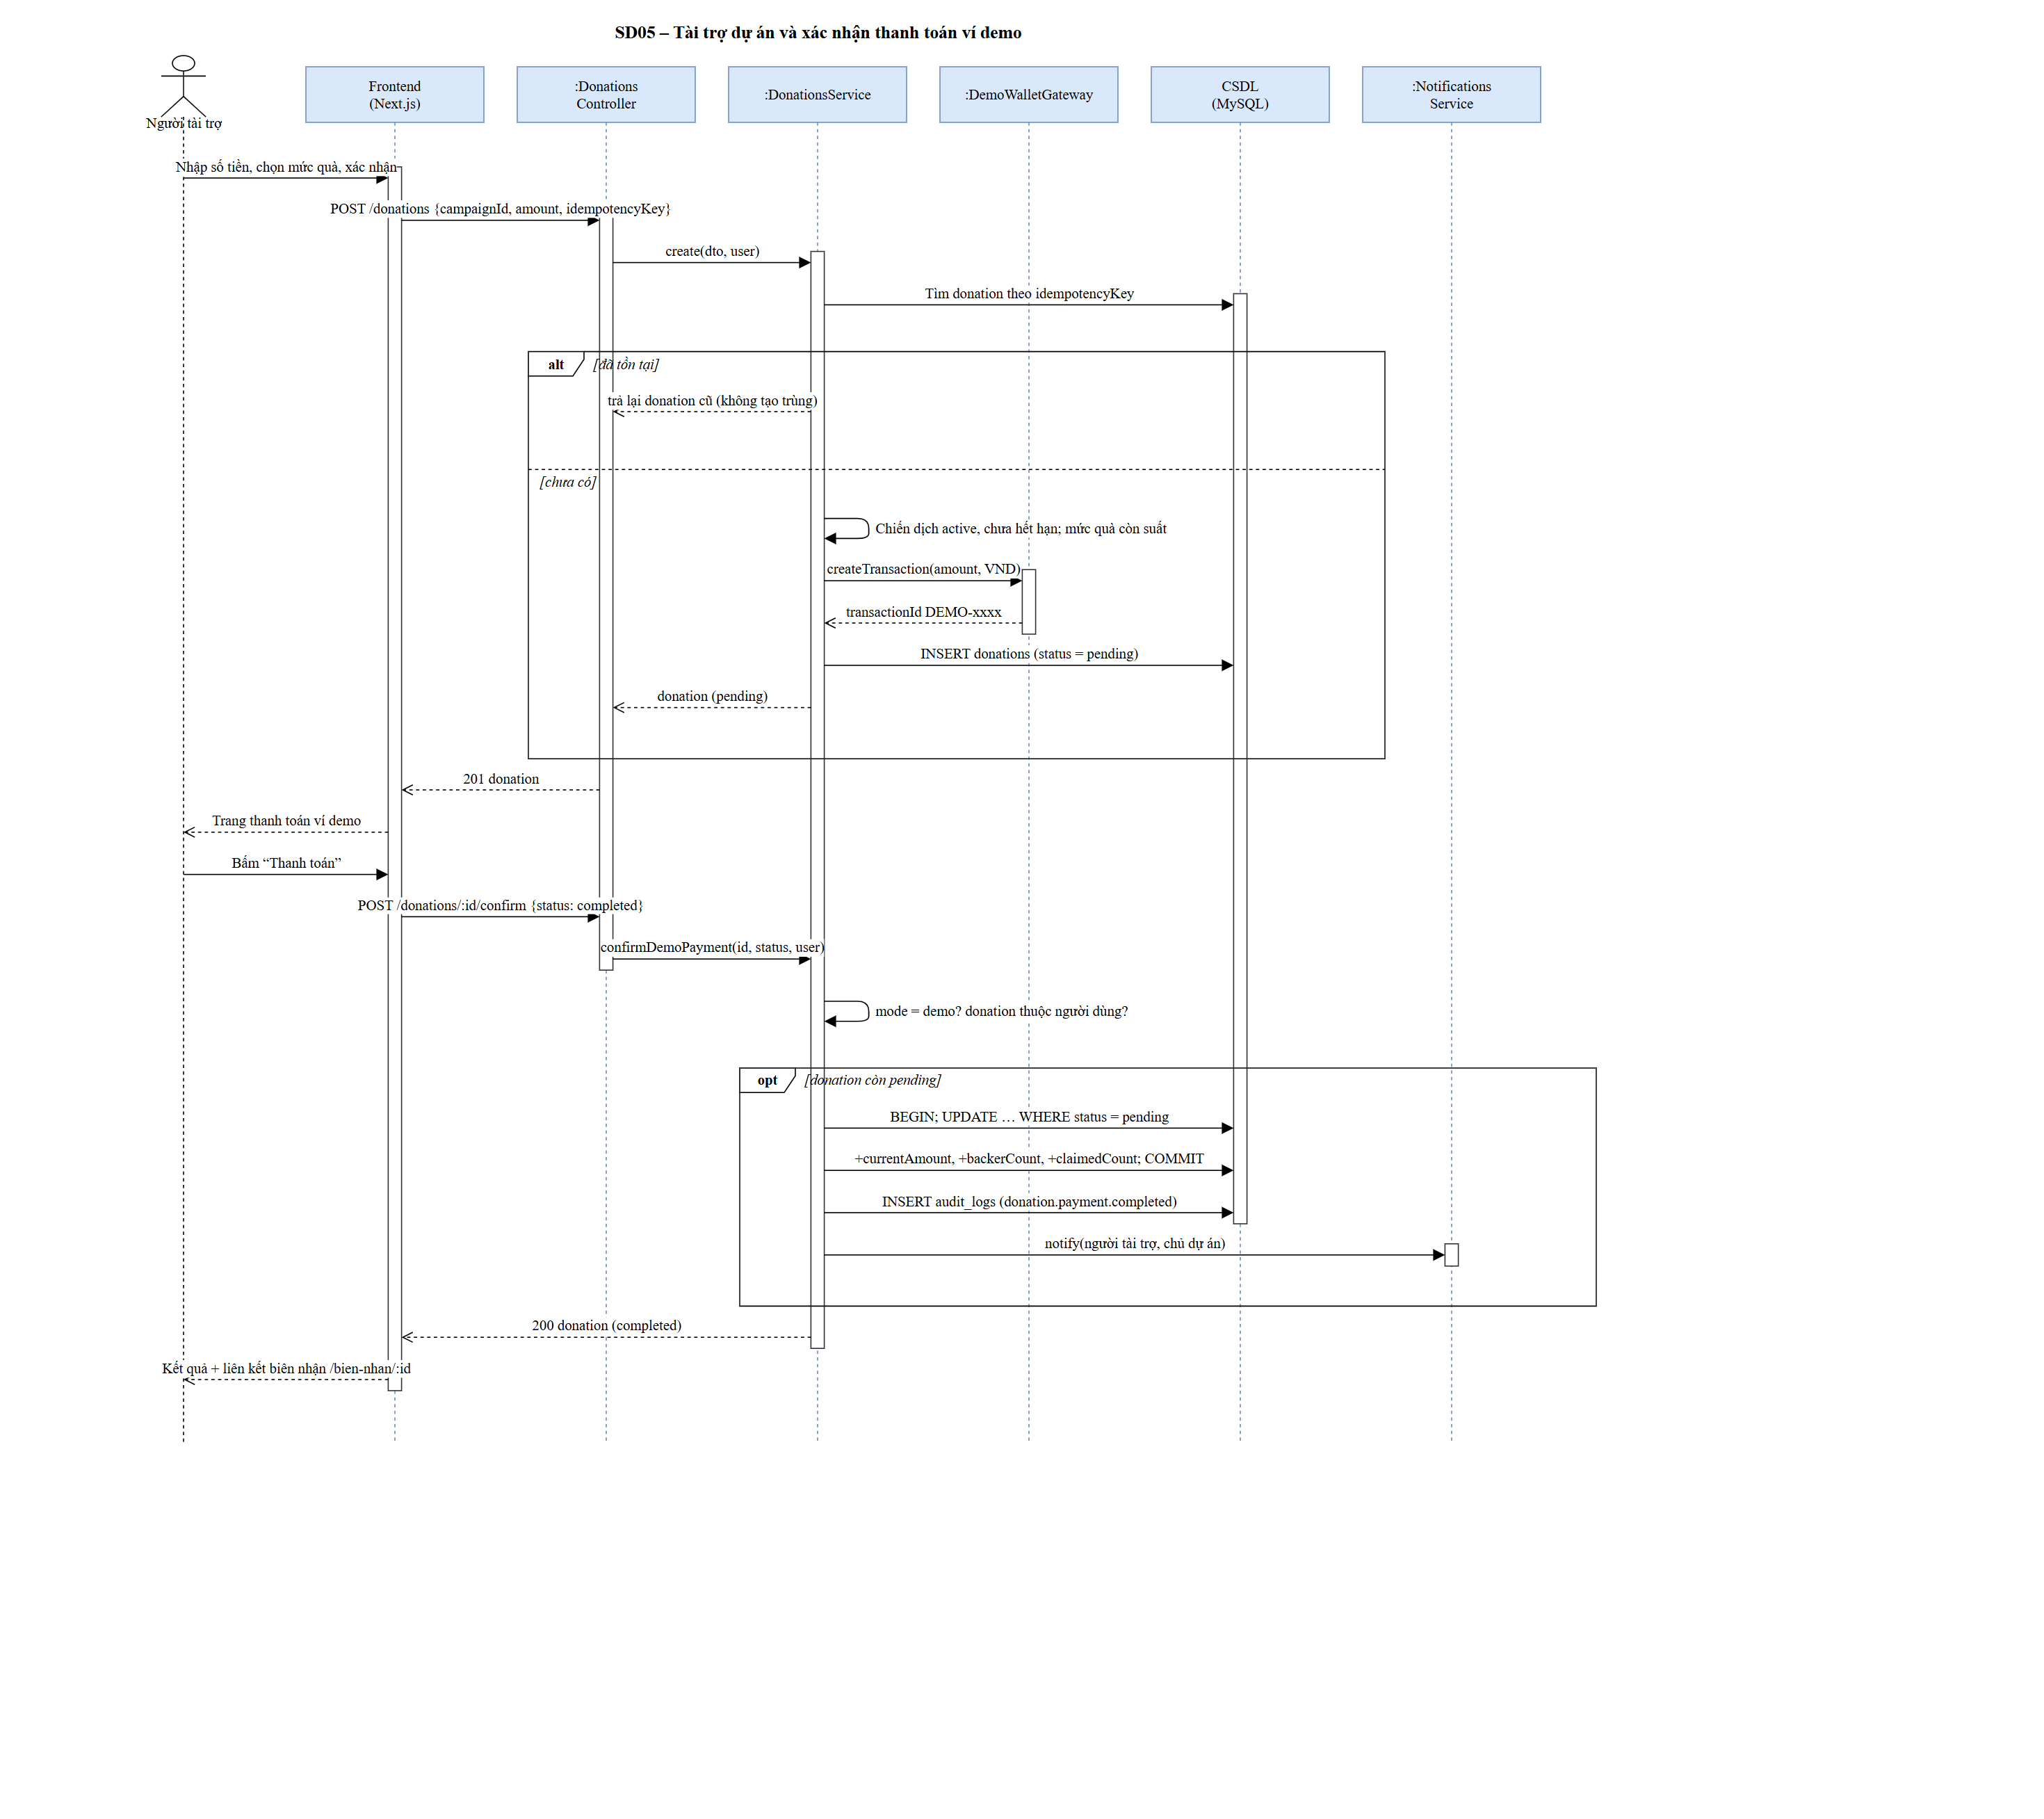
\includegraphics[width=0.95\textwidth,height=0.62\textheight,keepaspectratio]{image/SD05_TaiTroDuAn.png}
    \caption{Sơ đồ tuần tự luồng tài trợ và xác nhận thanh toán (SD05)}
    \label{fig:sd_tai_tro}
\end{figure}

\subsubsection{Gợi ý dự án và phương án dự phòng AI}

Kết quả AI có phương án dự phòng ở hai lớp:

\begin{enumerate}
    \item \textbf{Trong dịch vụ AI:} không nạp được file mô hình thì dùng luật kinh nghiệm; phản hồi mang cờ \texttt{fallback=true}.
    \item \textbf{Trong backend:} dịch vụ AI lỗi hoặc phản hồi quá 3 giây thì backend tự xếp hạng chiến dịch (gợi ý) hoặc chấm điểm bằng luật nghiệp vụ (cảnh báo rủi ro).
\end{enumerate}

Nhờ vậy tính năng nghiệp vụ không phụ thuộc vào việc AI sẵn sàng; giao diện ghi rõ kết quả đến từ mô hình hay từ luật dự phòng. Hành vi người dùng chỉ được gửi sang AI khi người dùng đã đồng ý cá nhân hóa. Trình tự được thể hiện trong Hình~\ref{fig:sd_goi_y}.

\begin{figure}[htbp]
    \centering
    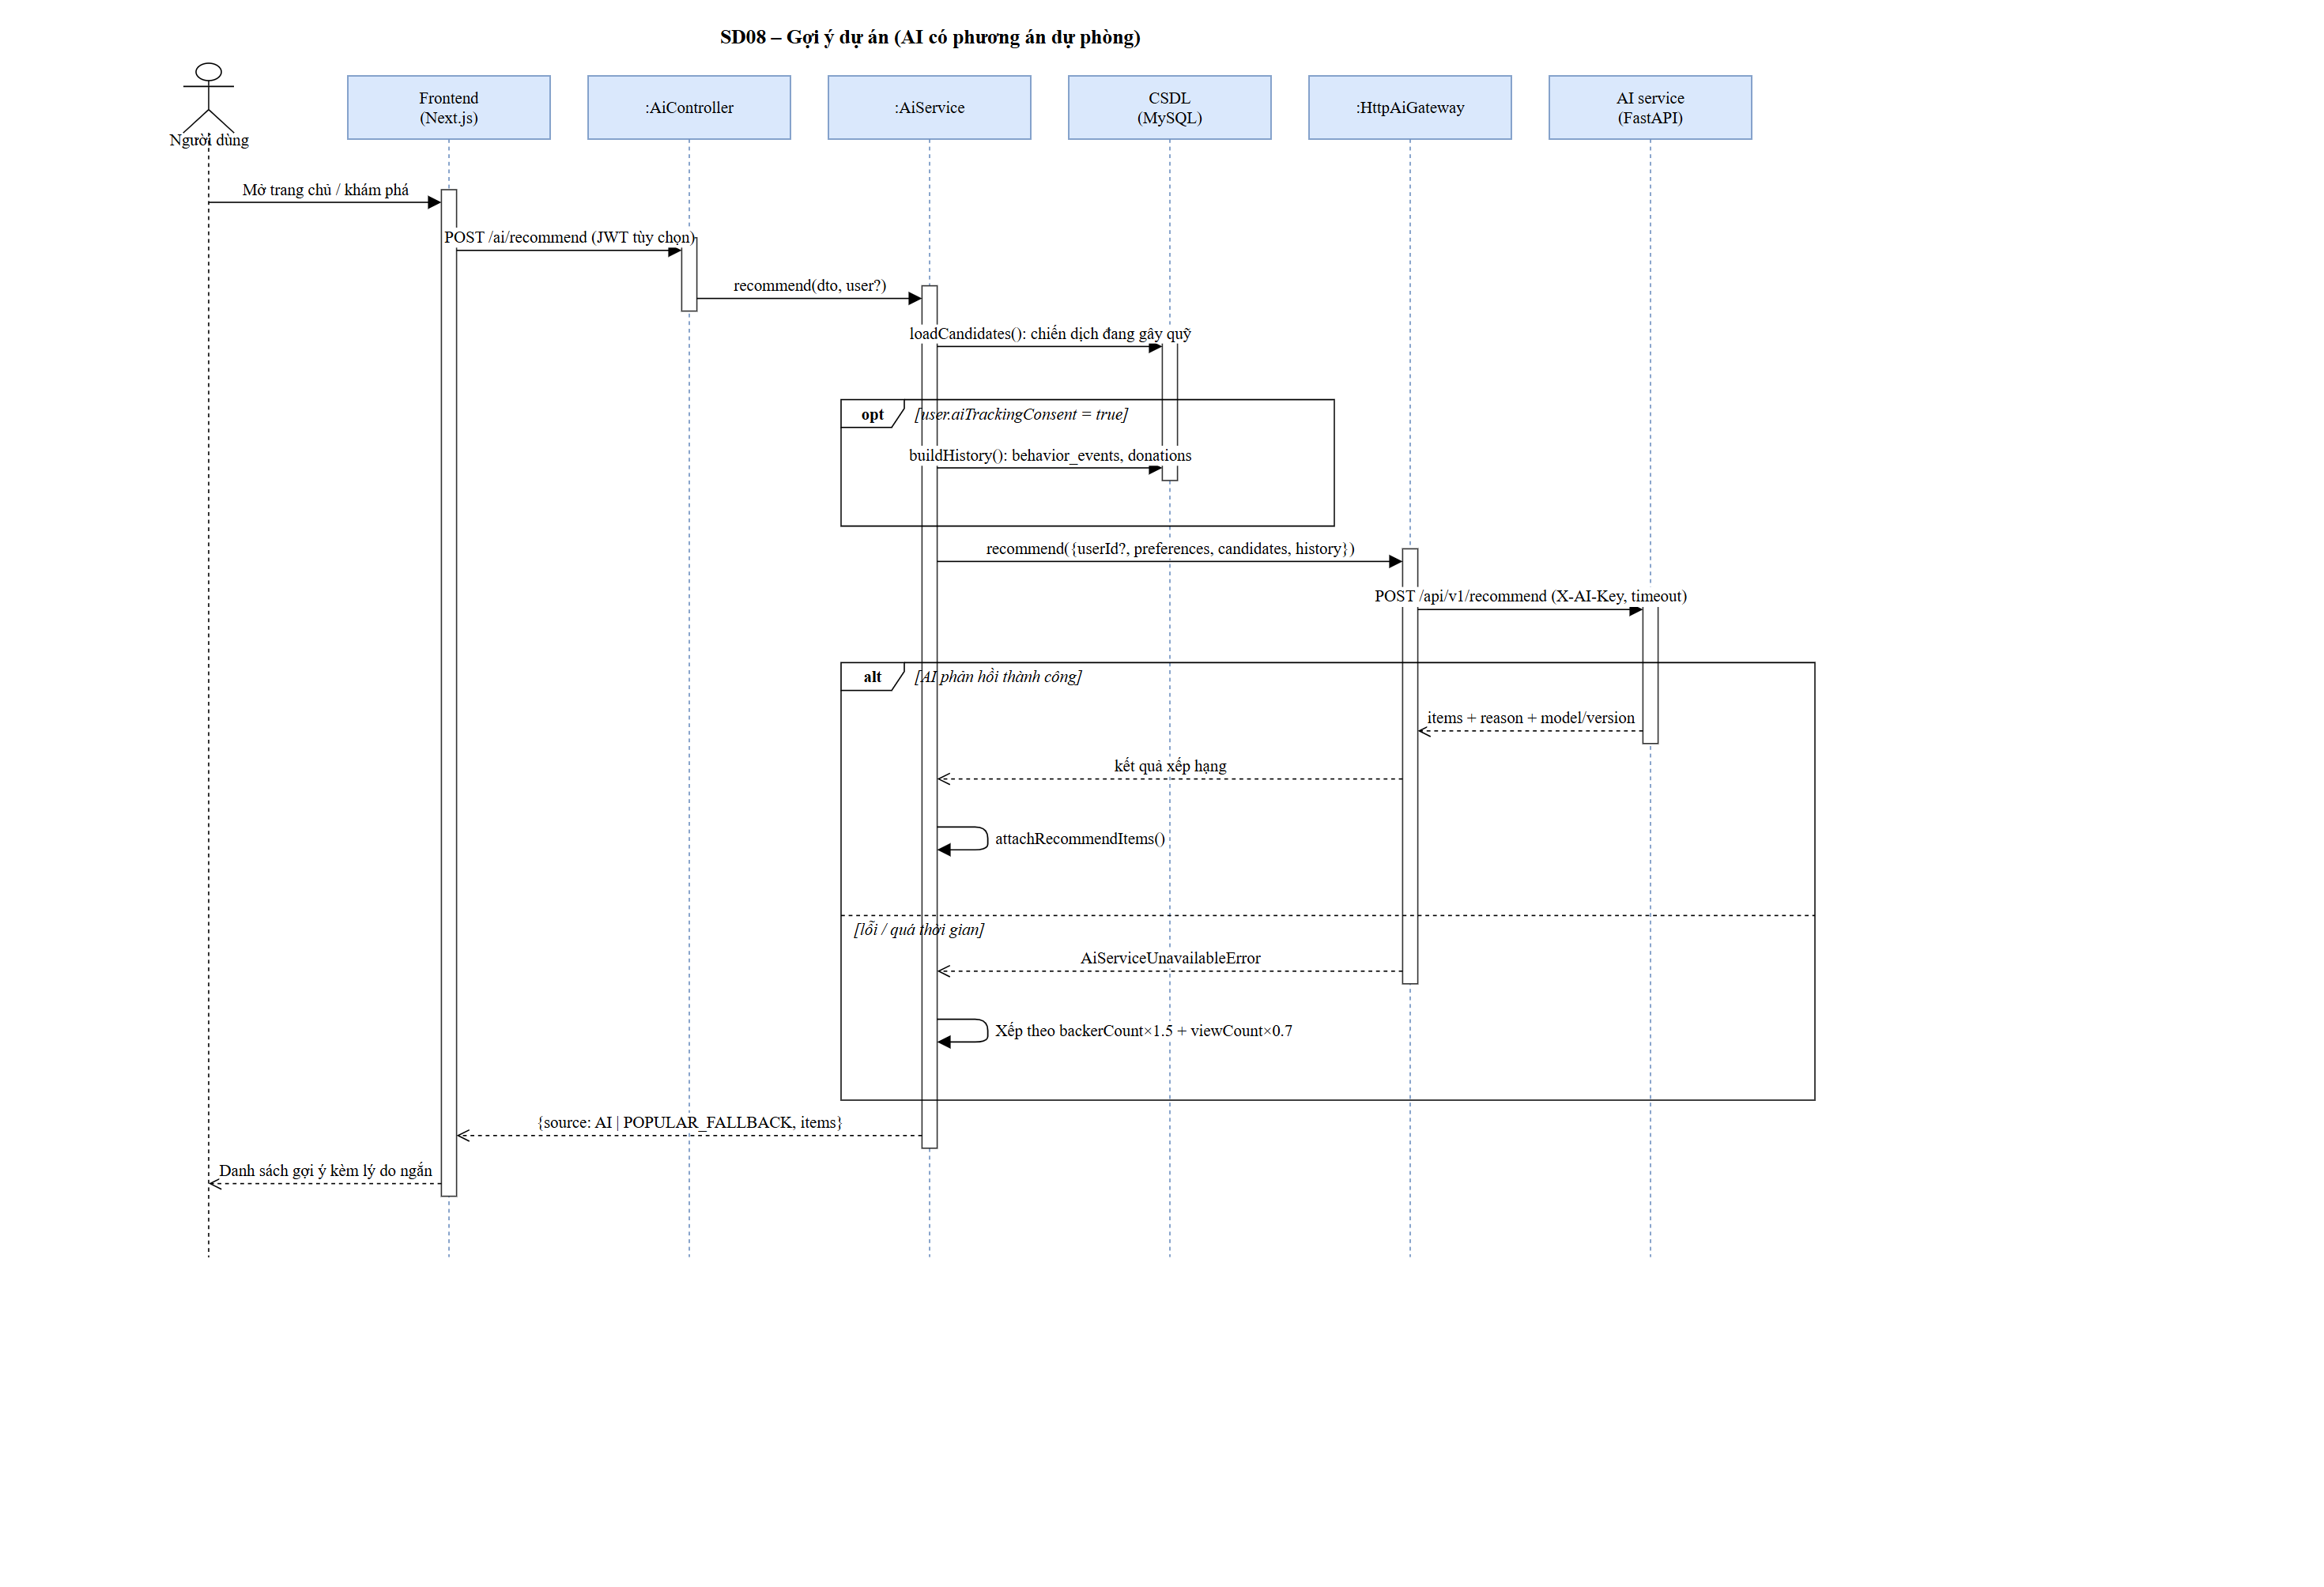
\includegraphics[width=0.95\textwidth,height=0.62\textheight,keepaspectratio]{image/SD08_GoiYDuAnAI.png}
    \caption{Sơ đồ tuần tự luồng gợi ý dự án có phương án dự phòng (SD08)}
    \label{fig:sd_goi_y}
\end{figure}

Các luồng còn lại (đăng ký, đăng nhập, xét duyệt chiến dịch, hoàn tiền, báo cáo vi phạm, tự động chốt chiến dịch) được mô tả trong bộ sơ đồ tuần tự SD01--SD11.

\subsection{Thiết kế bảo mật}

Mọi kiểm tra quyền và trạng thái tiền đều nằm ở backend. Các biện pháp bảo mật được tổ chức theo lớp như Bảng~\ref{tab:bao_mat}.

\begin{longtable}{|P{3.0cm}|p{10.8cm}|}
    \caption{Các biện pháp bảo mật theo lớp}
    \label{tab:bao_mat} \\
    \hline
    \textbf{Lớp} & \textbf{Biện pháp} \\
    \hline
    \endfirsthead
    \hline
    \textbf{Lớp} & \textbf{Biện pháp} \\
    \hline
    \endhead
    Xác thực & Mật khẩu băm bcrypt; JWT access và refresh token; refresh token xoay vòng, dùng lại token cũ sẽ vô hiệu mọi phiên; thu hồi token theo \texttt{jti} khi đăng xuất; khóa tạm tài khoản sau 5 lần đăng nhập sai trong 15 phút \\
    \hline
    Xác minh bổ sung & Mã OTP qua email trước thao tác nhạy cảm: đổi mật khẩu, yêu cầu hoàn tiền, quản trị viên duyệt hoàn tiền và xuất danh sách tài khoản nhận hoàn \\
    \hline
    Phân quyền & Theo vai trò (\texttt{user}, \texttt{campaign\_owner}, \texttt{admin}) và theo quyền sở hữu, kiểm tra ở máy chủ bằng \texttt{JwtAuthGuard}, \texttt{RolesGuard}; không thể tự đăng ký vai trò quản trị viên \\
    \hline
    Dữ liệu đầu vào & DTO và \texttt{ValidationPipe}; ORM tham số hóa truy vấn chống SQL injection; HTML mô tả được làm sạch ở máy chủ; kiểm tra loại và dung lượng ảnh tải lên \\
    \hline
    HTTP & \texttt{helmet}; CORS giới hạn nguồn qua \texttt{CORS\_ORIGINS}; \texttt{trust proxy} theo số lớp proxy; giới hạn tần suất bằng Redis \\
    \hline
    Thanh toán & Webhook ký HMAC, chống phát lại bằng timestamp; IPN SePay xác thực khóa và đối chiếu số tiền; idempotency key; cập nhật có điều kiện chống xử lý trùng; không lưu thông tin thẻ \\
    \hline
    Nội bộ & Dịch vụ AI yêu cầu header \texttt{X-AI-Key}, so sánh hằng thời gian; trên AWS chỉ load balancer được gọi vào các task \\
    \hline
    Dữ liệu cá nhân & Không trả \texttt{passwordHash} ra API; ảnh giấy phép tổ chức không lộ ra API công khai; hành vi chỉ được ghi khi người dùng đồng ý, rút lại thì xóa; file thống kê xuất ra đã ẩn danh \\
    \hline
    Truy vết & Nhật ký kiểm toán ghi thời điểm, người thực hiện, giá trị trước và sau; \texttt{X-Request-ID} đi xuyên suốt từ reverse proxy \\
    \hline
    Bí mật & Nằm trong biến môi trường; kho mã nguồn chỉ có \texttt{.env.example} với giá trị giữ chỗ \\
    \hline
\end{longtable}
